\section{Theorie}
\label{sec:Theorie}

% In knapper Form sind die physikalischen Grundlagen des Versuches, des Messverfahrens, sowie sämtliche für die Auswertung erforderlichen Gleichungen darzustellen. (Keine Herleitung)

% (eventuell die Aufgaben)

% Der Versuchsaufbau: Beschreibung des Versuchs und der Funktionsweise (mit Skizze/Bild/Foto)

\begin{figure}
    \centering
    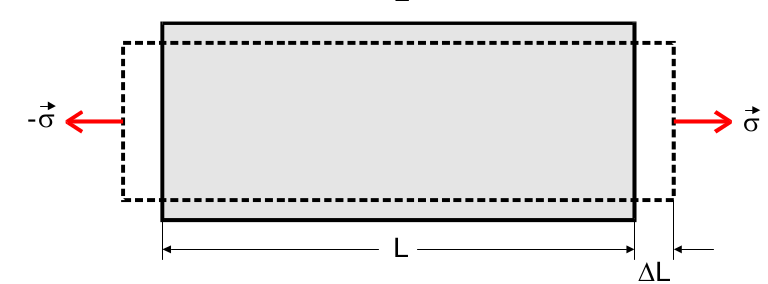
\includegraphics[width=\textwidth/2]{images/skizze_1.png}
    \caption{Dehnung einer stabförmigen Probe unter dem Einfluss einer Normalspannung\cite{V103}}
    \label{fig:skizze_1}
\end{figure}
Wenn ein Körper deformiert wird und diese Deformation den elastischen Bereich nicht überschreitet, wird der Zusammenhang zwischen Spannung $\sigma$ und Deformationsverhältnis $\Delta L / L$ durch das Hookesche Gesetz
\begin{equation}
    \sigma = E \, \frac{\Delta L}{L}
    \label{eq:hookesches_gesetz}
\end{equation}
beschrieben. \cite{V103}
Wobei $E$ der Elastizitätsmodul und somit eine Materialkonstante ist.
 
\begin{figure}
    \centering
    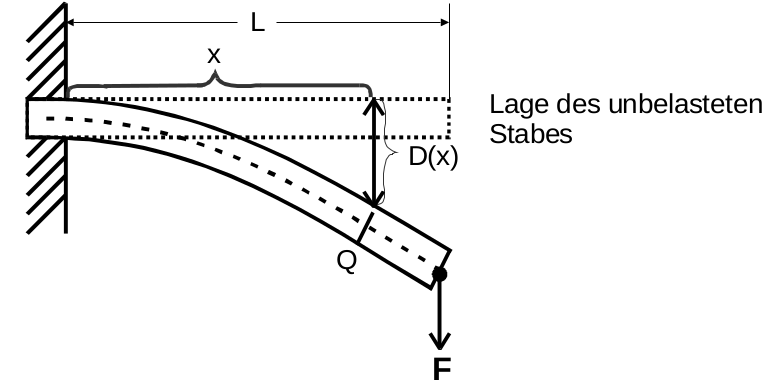
\includegraphics[width=\textwidth/2]{images/skizze_2.png}
    \caption{Skizze eines gebogenen Stabes\cite{V103}}
    \label{fig:skizze_2}
\end{figure}
Nun kann die Biegung eines Stabes durch die Kraft $F$ auch als Dehnung angesehen werden, da eine Seite gedehnt und die andere Seite gestaucht wird.
Zwischen diesen Seiten liegt eine Fläche, welche weder gestreckt noch gestaucht ist.
Diese Fläche wird neutrale Faser genannt. Nun sei $Q$ die Querschnittsfläche vom Stab und $D(x)$ der Abstand des durchgebogenen Stabes zum Ausgangsstab.(siehe \autoref{fig:skizze_2})
Dann kann das an $Q$ angreifende Drehmoment
\begin{equation}
    M_\sigma = \int_Q y\sigma(y)\dif{q}
    \label{eq:drehmoment_sigma}
\end{equation}
gleich dem Drehmoment der wirkenden Kraft $F$ gesetzt werden, um durch Umformungen eine Gleichung für $D(x)$ zu bestimmen.
Dazu wird außerdem die Definition des Flächenträgheitsmoments
\begin{equation}
    I = \int_Q y^2 \dif{q}
    \label{eq:flächentragheitsmoment}
\end{equation}
und das Hookesche Gesetz verwendet. Wobei $y$ der Abstand des infinitesimalen Flächenelements $\dif{q}$ zur neutralen Faser ist.

Für die einseitige Einspannung des Stabes ergibt sich durch das Drehmoment der Kraft
\begin{equation}
    M_F = F (L-x)
    \label{eq:drehmoment_einseitig}
\end{equation}
die Gleichung für die Durchbiegung
\begin{equation}
    D(x) = \frac{F}{2EI} \left( Lx^2 - \frac{x^3}{3} \right). \: \text{\cite{V103}}
    \label{eq:durchbiegung_einseitig}
\end{equation}
Hiermit kann im Versuch der Elastizitätsmodul bestimmt werden.

Eine weitere Möglichkeit ergibt sich, wenn der Stab beidseitig eingespannt wird. Nun ist das Drehmoment der Kraft
\begin{equation}
    M_F = 
    \begin{cases}
        -\frac{F}{2}x, & 0 \leq x \leq L/2 \\
        \\
        -\frac{F}{2}(L-x) & L/2 \leq x \leq L
    \end{cases}
    \label{eq:drehmoment_beidseitig}
\end{equation}
und für die Durchbiegung ergibt sich
\begin{equation}
    D(x) = 
    \begin{cases}
        \frac{F}{48EI} \left( 3L^2x - 4x^3 \right), & 0 \leq x \leq L/2 \\
        \\
        \frac{F}{48EI} \left( 4x^3 - 12Lx^2 + 9L^2x - L^3 \right), & L/2 \leq x \leq L
    \end{cases}
    . \: \text{\cite{V103}}
    \label{eq:durchbiegung_beidseitig}
\end{equation}
